\newpage
\refstepcounter{section}
%Add Image
\vspace*{-40mm} %Make image have no top margin
\begin{tikzpicture}
\node[inner sep=0pt] (x) at (0,0)
    {\hspace{-87mm}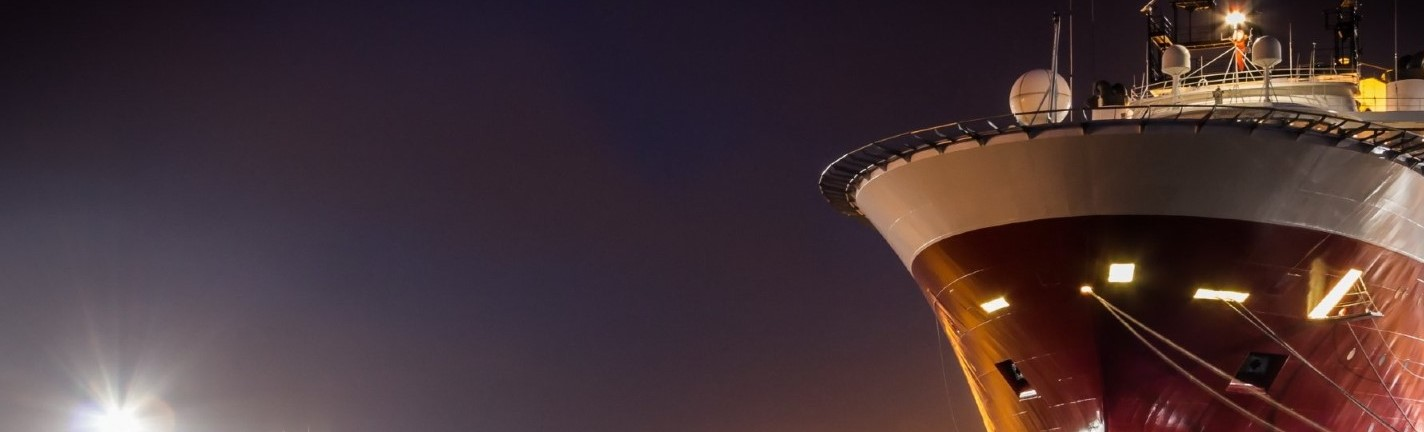
\includegraphics[width=\paperwidth]{sectionimage4.jpg}};
\node[text width=10in] (Z) at (0,-1) {\color{white}\headingfont\Large\bfseries\uppercase{\hspace{-0.7cm}\thesection\hspace{0.5cm}Conclusions \& Recommendations}};
\end{tikzpicture}
%Modify TOC
\addcontentsline{toc}{section}{\protect\numberline{\thesection}Conclusions \& Recommendations}
  \sectionmark{Conclusions \& Recommendations}
\vspace{-2mm}

\subsection*{Conclusion:}

This feasibility study was undertaken to assess if relocation of the PoA would benefit Auckland city and the New Zealand Economy. With an increase in freight demand in the future due to larger ships and increasing population, the PoA will not meet demand. Relocation of the PoA would provide available land for real estate and other community based infrastructure, which can provide economic growth for Auckland. Traffic congestion will also be reduced due to fewer container trucks on Auckland roads. 
\\Existing ports and possible areas where the PoA could be repositioned were investigated, these were assessed and compared to find a best-fit solution. This solution will meet the stakeholder requirements and should be viable to implement (with regards to cost and efficiency).
\\The best fit solution chosen is relocating 80\% of the PoA’s shipping traffic to the PoT and leaving PoA at 20\% of its current shipping traffic. The proposed plan will span between 25 years and will involve:
\begin{itemize}[noitemsep]
    \vspace{-2mm}
    \item{Development of roading of SH 29 and changing the route of container trucks from Auckland to Tauranga to use SH 1 and 29}
    \item{2 stage expansion of PoT to accommodate the relocation}
    \item{Development of the East Coast Main Trunk rail line}
\end{itemize}
This solution was chosen as it is the most economically feasible option. From the CBA, the cost-benefit ratio of this solution was calculated to be 1.5 suggesting that benefits received by the project outweigh the cost and the project is worthwhile.
\subsection*{Recommendations:}
303 Consulting recommends the best fit solution should be approved by the government as it will benefit New Zealand economically, socially and environmentally. 
\\Incorporating the Ruakura Inland Freight Hub within the operations of freight transport between PoA and PoT is also recommended as it can relieve some of the freight storage in these ports. This solution will also further develop the AKL to HTN and HTN to TRG links of the ‘Golden Triangle’ in the upper North Island. Further planning to be conducted would include a more comprehensive analysis of the major stakeholders, a more detailed plan to allocate shipping traffic over the transition period, and a more detailed economic analysis. From this feasibility study, 303 consulting considers the best-fit option to be feasible, and a viable solution to the requirements presented and recommends further investigation into this project.

\clearpage